\documentclass{beamer}
\usepackage[utf8]{inputenc}

\usetheme{Madrid}
\usecolortheme{default}
\usepackage{amsmath,amssymb,amsfonts,amsthm}
\usepackage{txfonts}
\usepackage{tkz-euclide}
\usepackage{listings}
\usepackage{adjustbox}
\usepackage{array}
\usepackage{tabularx}
\usepackage{gvv}
\usepackage{lmodern}
\usepackage{circuitikz}
\usepackage{tikz}
\usepackage{graphicx}

\setbeamertemplate{page number in head/foot}[totalframenumber]

\usepackage{tcolorbox}
\tcbuselibrary{minted,breakable,xparse,skins}



\definecolor{bg}{gray}{0.95}
\DeclareTCBListing{mintedbox}{O{}m!O{}}{%
	breakable=true,
	listing engine=minted,
	listing only,
	minted language=#2,
	minted style=default,
	minted options={%
		linenos,
		gobble=0,
		breaklines=true,
		breakafter=,,
		fontsize=\small,
		numbersep=8pt,
		#1},
	boxsep=0pt,
	left skip=0pt,
	right skip=0pt,
	left=25pt,
	right=0pt,
	top=3pt,
	bottom=3pt,
	arc=5pt,
	leftrule=0pt,
	rightrule=0pt,
	bottomrule=2pt,
	toprule=2pt,
	colback=bg,
	colframe=orange!70,
	enhanced,
	overlay={%
		\begin{tcbclipinterior}
			\fill[orange!20!white] (frame.south west) rectangle ([xshift=20pt]frame.north west);
	\end{tcbclipinterior}},
	#3,
}
\lstset{
	language=C,
	basicstyle=\ttfamily\small,
	keywordstyle=\color{blue},
	stringstyle=\color{orange},
	commentstyle=\color{green!60!black},
	numbers=left,
	numberstyle=\tiny\color{gray},
	breaklines=true,
	showstringspaces=false,
}
\begin{document}

\title 
{1.9.29}
\date{1 September,2025}

\author 
{Naman Kumar-EE25BTECH11041}
\graphicspath{./figs}


\frame{\titlepage}
\begin{frame}{Question}
Find the value of y for which the distance between the points $\Vec{A}\brak{3,-1}$ and $\Vec{B}\brak{11,y}$ is 10 units.
\end{frame}
\begin{frame}{Equation Used}
\begin{equation}
    \text{Distance }=\lVert \vec{A}-\vec{B}\rVert= \sqrt{(\vec{A}-\vec{B})^{T}(\vec{A}-\vec{B})} \label{eq1}
\end{equation}
\end{frame}
\begin{frame}{Solution}
\begin{align}
    \vec{A}-\vec{B}=\begin{myvec}{3-11\\-1-y} \end{myvec}
\end{align}
Next
\begin{align}
    (\vec{A}-\vec{B})^{T}(\vec{A}-\vec{B}) = \begin{myvec}{3-11&-1-y} \end{myvec} \begin{myvec}{3-11\\-1-y} \end{myvec}
\end{align}
\end{frame}
\begin{frame}
Putting values in equation \eqref{eq1} 
\begin{align}
    \sqrt{(3-11)^2+(-1-y)^2}=10\\
    (3-11)^2+(-1-y)^2=100\\
    64+1+y^2+2y=100\\
    y^2+2y-35=0\\
    (y+7)(y-5)=0\\
    y=-7 \text{ or } 5 
\end{align}
Therefore, there are two possible values of $\Vec{B}\brak{11,5}$ or $\Vec{B}\brak{11,-7}$
\end{frame}
\begin{frame}[fragile]
\frametitle{C code}
\begin{lstlisting}
#include <stdio.h>
#include <math.h>

// Function to compute dot product
void dot_product(double vector1[], double vector2[], int size, double* result) {
    *result = 0.0;
    for (int i = 0; i < size; i++) {
        *result += vector1[i] * vector2[i];
    }
}
\end{lstlisting}
\end{frame}
\begin{frame}[fragile]
\frametitle{C code}
\begin{lstlisting}


// Function to compute squared distance between two 2D points using dot product
void distance_squared(double A[2], double B[2], double* result) {
    double AB[2];
    AB[0] = B[0] - A[0];   // x2 - x1
    AB[1] = B[1] - A[1];   // y2 - y1
    dot_product(AB, AB, 2, result); // AB · AB
}
\end{lstlisting}
\end{frame}
\begin{frame}[fragile]
\frametitle{Python Code through Shared obejct}
\begin{lstlisting}
import ctypes
import numpy as np
import matplotlib.pyplot as plt
import math

# Load shared library
lib = ctypes.CDLL("./main.so")

# Define signatures
lib.distance_squared.argtypes = [
    np.ctypeslib.ndpointer(dtype=np.float64, flags="C_CONTIGUOUS"),
    np.ctypeslib.ndpointer(dtype=np.float64, flags="C_CONTIGUOUS"),
    ctypes.POINTER(ctypes.c_double)
]
\end{lstlisting}
\end{frame}
\begin{frame}[fragile]
\frametitle{Python Code through Shared obejct}
\begin{lstlisting}
lib.distance_squared.restype = None

def distance_squared(A, B):
    res = ctypes.c_double()
    lib.distance_squared(A, B, ctypes.byref(res))
    return res.value

# Point A
A = np.array([3.0, -1.0], dtype=np.float64)

# B points from solving equation (y = 5 or y = -7)
solutions = [5.0, -7.0]
points = []

for yB in solutions:
    B = np.array([11.0, yB], dtype=np.float64)
    d2 = distance_squared(A, B)
    d = math.sqrt(d2)
\end{lstlisting}
\end{frame}
\begin{frame}[fragile]
\frametitle{Python Code through Shared obejct}
\begin{lstlisting}
    print(f"For y = {yB}, distance AB = {d}")
    points.append(B)
# --- Plot ---
plt.figure(figsize=(6,6))
plt.scatter(A[0], A[1], color="red")
plt.text(A[0]+0.2, A[1]+0.2, "A(3, -1)", color="red", fontsize=10)

for i, B in enumerate(points, start=1):
    plt.scatter(B[0], B[1], color="blue")
    plt.text(B[0]+0.2, B[1]+0.2, f"B{ i }(11, {int(B[1])})", color="blue", fontsize=10)
    plt.plot([A[0], B[0]], [A[1], B[1]], linestyle="--")
\end{lstlisting}
\end{frame}
\begin{frame}[fragile]
\frametitle{Python Code through Shared obejct}
\begin{lstlisting}
plt.xlabel("X-axis")
plt.ylabel("Y-axis")
plt.title("Points A and B with distance 10 (using C distance_squared)")
plt.grid(True)
plt.axis("equal")
plt.show()
\end{lstlisting}
\end{frame}
\begin{frame}[fragile]
\frametitle{Direct python Code}
\begin{lstlisting}
import numpy as np
import matplotlib.pyplot as plt
import math

# --- 1. Define the given points and distance ---
p_a = np.array([3, -1])
x_b = 11
distance = 10

# --- 2. Solve for y ---
# We have the equation: distance^2 = (x_b - p_a[0])^2 + (y - p_a[1])^2
# 10^2 = (11 - 3)^2 + (y - (-1))^2
# 100 = 8^2 + (y + 1)^2
# 100 = 64 + (y + 1)^2
# 36 = (y + 1)^2
# So, y + 1 = +/- 6

# First solution for y
y1 = 6 - 1
\end{lstlisting}
\end{frame}
\begin{frame}[fragile]
\frametitle{Direct python Code}
\begin{lstlisting}
# Second solution for y
y2 = -6 - 1
p_b1 = np.array([x_b, y1])
p_b2 = np.array([x_b, y2])

# --- 3. Plot the results ---
# Create a figure and axis for the plot
fig, ax = plt.subplots(figsize=(10, 10))

# Plot the points A, B1, and B2
ax.scatter(p_a[0], p_a[1], color='red', s=100, zorder=5)
ax.scatter(p_b1[0], p_b1[1], color='blue', s=100, zorder=5)
ax.scatter(p_b2[0], p_b2[1], color='green', s=100, zorder=5)
\end{lstlisting}
\end{frame}
\begin{frame}[fragile]
\frametitle{Direct python Code}
\begin{lstlisting}
# Annotate the points directly on the graph
ax.text(p_a[0] + 0.3, p_a[1], f'A ({p_a[0]}, {p_a[1]})', fontsize=12, verticalalignment='center', color='red')
ax.text(p_b1[0] + 0.3, p_b1[1], f'B1 ({p_b1[0]}, {p_b1[1]})', fontsize=12, verticalalignment='center', color='blue')
ax.text(p_b2[0] + 0.3, p_b2[1], f'B2 ({p_b2[0]}, {p_b2[1]})', fontsize=12, verticalalignment='center', color='green')

# Draw the lines representing the distance
ax.plot([p_a[0], p_b1[0]], [p_a[1], p_b1[1]], 'b--', label=f'Distance = {distance} units')
\end{lstlisting}
\end{frame}
\begin{frame}[fragile]
\frametitle{Direct python Code}
\begin{lstlisting}
ax.plot([p_a[0], p_b2[0]], [p_a[1], p_b2[1]], 'g--')

# --- Visualization Aid: Draw a circle centered at A with radius 10 ---
# The solution points B1 and B2 must lie on this circle.
circle = plt.Circle(p_a, distance, color='red', fill=False, linestyle=':', alpha=0.5)
ax.add_artist(circle)

# --- Visualization Aid: Draw the vertical line x = 11 ---
\end{lstlisting}
\end{frame}
\begin{frame}[fragile]
\frametitle{Direct python Code}
\begin{lstlisting}
# Point B must lie on this line.
ax.axvline(x=x_b, color='purple', linestyle='-.', alpha=0.5)

# --- 4. Formatting the plot ---
ax.set_title('Geometric Solution for the Distance Problem', fontsize=16)
ax.set_xlabel('X-axis', fontsize=12)
ax.set_ylabel('Y-axis', fontsize=12)

# Set equal aspect ratio to ensure the circle is not distorted
ax.set_aspect('equal', adjustable='box')

# Add grid and legend
ax.grid(True, which='both', linestyle='--', linewidth=0.5)
ax.legend(fontsize=10)
\end{lstlisting}
\end{frame}
\begin{frame}[fragile]
\frametitle{Direct python Code}
\begin{lstlisting}
# Set axis limits to give some padding around the points
plt.xlim(p_a[0] - distance - 2, p_a[0] + distance + 2)
plt.ylim(p_a[1] - distance - 2, p_a[1] + distance + 2)

# Save the plot as a PNG file
plt.savefig('distance_plot.png')

# Show the plot
plt.show()
\end{lstlisting}
\end{frame}
\begin{frame}{Figure}
    \begin{figure}[H]
        \centering
        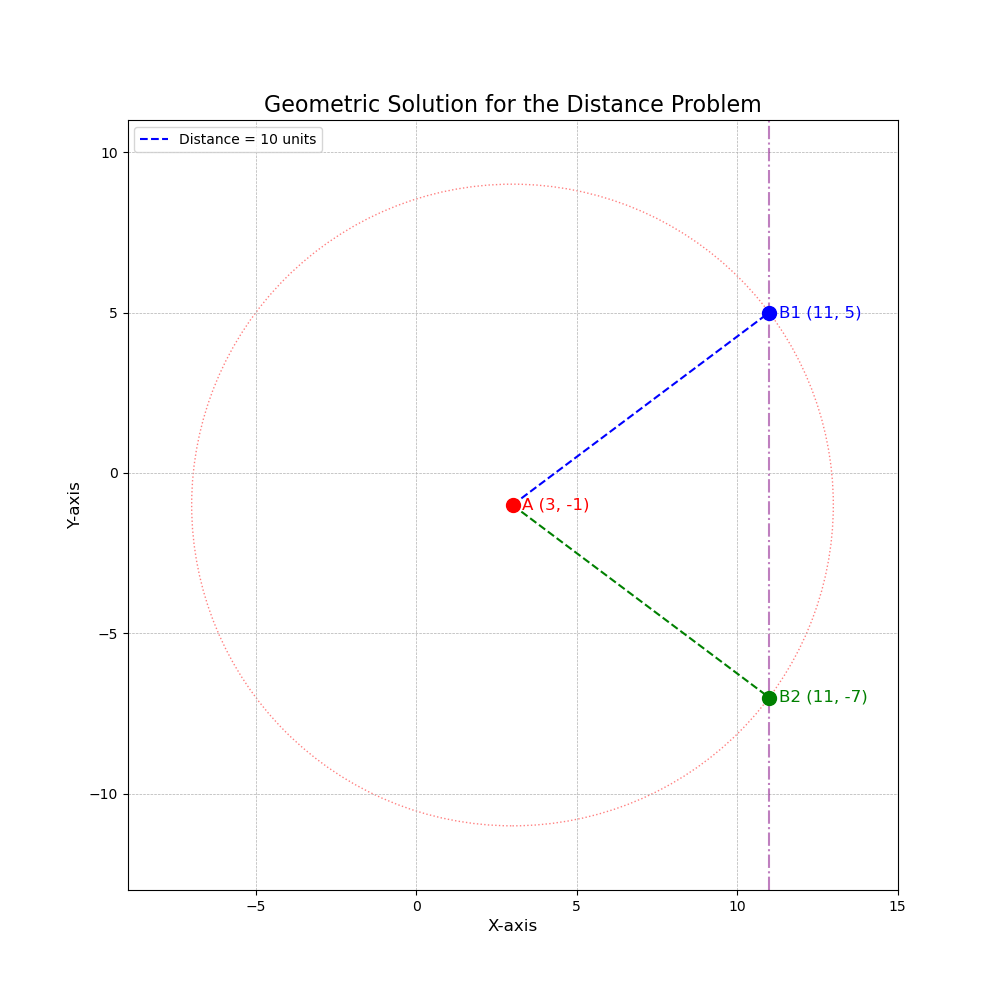
\includegraphics[width=0.6\columnwidth]{figs/distance_plot.png}
    \end{figure}
\end{frame}
\end{document}